%!Mode:: "TeX:UTF-8"
\documentclass[a4paper,11pt,UTF8]{ctexart}

\usepackage{indentfirst} %缩进
\usepackage{xeCJK}    %使用系统字体
\usepackage{fancyhdr} %自定义页眉页脚
\pagestyle{empty}                   %不设置页眉页脚
\usepackage{amsmath, amsthm, amssymb, amsfonts} %数学公式
\usepackage[a4paper,left=3cm,right=3cm,top=3cm,bottom=3cm]{geometry}
%\usepackage[tmargin=1in,bmargin=1in,lmargin=1.25in,rmargin=1.25in]{geometry}.
\usepackage{booktabs} %插入表格
\usepackage[section]{placeins} %避免浮动
\usepackage{listings} %插入代码
\usepackage{ctex}     %中文宏包
\usepackage[svgnames, table]{xcolor} %彩色表格
\usepackage{algorithm}          %伪代码
\usepackage{algorithmicx}
\usepackage{algpseudocode}
\usepackage{algorithm,algpseudocode,float}
\usepackage{lipsum}
\usepackage{enumitem}           %调整列举环境
\usepackage{url}
\usepackage{fontspec,xunicode}
\defaultfontfeatures{Mapping=tex-text} %如果没有它,会有一些 tex 特殊字符无法正常使用,比如连字符。

\usepackage{graphicx}
\graphicspath{{imgs/}}

%%%%%%%%%%%%%%%%%%%%%%%%%%%%%%%%%%%%%%%%%%%%%%%%%%%%%%%%%%%%%%%%
% 缩进及行间距
%%%%%%%%%%%%%%%%%%%%%%%%%%%%%%%%%%%%%%%%%%%%%%%%%%%%%%%%%%%%%%%%
\setlength{\parindent}{22pt} %重新定义缩进长度
\setlength{\baselineskip}{20pt}  %定义行间距
%\renewcommand{\baselinestretch}{1.1} %定义行间距

%%%%%%%%%%%%%%%%%%%%%%%%%%%%%%%%%%%%%%%%%%%%%%%%%%%%%%%%%%%%%%%%
% 列表设置
%%%%%%%%%%%%%%%%%%%%%%%%%%%%%%%%%%%%%%%%%%%%%%%%%%%%%%%%%%%%%%%%
\setenumerate{fullwidth,itemindent=\parindent,listparindent=\parindent,itemsep=0ex,partopsep=0pt,parsep=0ex}
\setenumerate[2]{label=\alph*),leftmargin=1.5em}  %二级item设置
\setitemize{itemindent=38pt,leftmargin=0pt,itemsep=-0.4ex,listparindent=26pt,partopsep=0pt,parsep=0.5ex,topsep=-0.25ex}
\setdescription{itemindent=38pt,leftmargin=0pt,itemsep=-0.4ex,listparindent=26pt,partopsep=0pt,parsep=0.5ex,topsep=-0.25ex}

%%%%%%%%%%%%%%%%%%%%%%%%%%%%%%%%%%%%%%%%%%%%%%%%%%%%%%%%%%%%%%%%
% 图的标题行间距设置
%%%%%%%%%%%%%%%%%%%%%%%%%%%%%%%%%%%%%%%%%%%%%%%%%%%%%%%%%%%%%%%%
\newcommand{\bottomcaption}{%
\setlength{\abovecaptionskip}{6pt}%
\setlength{\belowcaptionskip}{6pt}%
\caption}


%%%%%%%%%%%%%%%%%%%%%%%%%%%%%%%%%%%%%%%%%%%%%%%%%%%%%%%%%%%%%%%%
% 字体定义
%%%%%%%%%%%%%%%%%%%%%%%%%%%%%%%%%%%%%%%%%%%%%%%%%%%%%%%%%%%%%%%%
\setmainfont{Times New Roman}  %默认英文字体.serif是有衬线字体sans serif无衬线字体
\setmonofont{Consolas}
\setCJKmainfont[ItalicFont={楷体}, BoldFont={黑体}]{宋体}%衬线字体 缺省中文字体为
\setCJKsansfont{黑体}
\punctstyle{hangmobanjiao}
%-----------------------xeCJK下设置中文字体------------------------------%
\setCJKfamilyfont{song}{SimSun}                             %宋体 song
\newcommand{\song}{\CJKfamily{song}}
\setCJKfamilyfont{fs}{FangSong}                      %仿宋  fs
\newcommand{\fs}{\CJKfamily{fs}}
\setCJKfamilyfont{ktgb}{KaiTi}                      %楷体2312 ktgb
\newcommand{\ktgb}{\CJKfamily{ktgb}}
\setCJKfamilyfont{yh}{Microsoft YaHei}                    %微软雅黑 yh
\newcommand{\yh}{\CJKfamily{yh}}
\setCJKfamilyfont{hei}{SimHei}                              %黑体  hei
\newcommand{\hei}{\CJKfamily{hei}}
\setCJKfamilyfont{hwxk}{STXingkai}                                %华文行楷  hwxk
\newcommand{\hwxk}{\CJKfamily{hwxk}}
%------------------------------设置字体大小------------------------%
\newcommand{\shiyanbaogao}{\fontsize{36pt}{\baselineskip}\selectfont}
\newcommand{\chuhao}{\fontsize{42pt}{\baselineskip}\selectfont}     %初号
\newcommand{\xiaochuhao}{\fontsize{36pt}{\baselineskip}\selectfont} %小初号
\newcommand{\yihao}{\fontsize{28pt}{\baselineskip}\selectfont}      %一号
\newcommand{\erhao}{\fontsize{21pt}{\baselineskip}\selectfont}      %二号
\newcommand{\xiaoerhao}{\fontsize{18pt}{\baselineskip}\selectfont}  %小二号
\newcommand{\sanhao}{\fontsize{15.75pt}{\baselineskip}\selectfont}  %三号
\newcommand{\sihao}{\fontsize{14pt}{\baselineskip}\selectfont}       %四号
\newcommand{\xiaosihao}{\fontsize{12pt}{\baselineskip}\selectfont}  %小四号
\newcommand{\wuhao}{\fontsize{10.5pt}{\baselineskip}\selectfont}    %五号
\newcommand{\xiaowuhao}{\fontsize{9pt}{\baselineskip}\selectfont}   %小五号
\newcommand{\liuhao}{\fontsize{7.875pt}{\baselineskip}\selectfont}  %六号
\newcommand{\qihao}{\fontsize{5.25pt}{\baselineskip}\selectfont}    %七号

%%%%%%%%%%%%%%%%%%%%%%%%%%%%%%%%%%%%%%%%%%%%%%%%%%%%%%%%%%%%%%%%
% 图题字体大小相同
%%%%%%%%%%%%%%%%%%%%%%%%%%%%%%%%%%%%%%%%%%%%%%%%%%%%%%%%%%%%%%%%
\usepackage{caption}
\captionsetup{font={footnotesize}}   % footnotesize = 9pt
\captionsetup[lstlisting]{font={footnotesize}}

%%%%%%%%%%%%%%%%%%%%%%%%%%%%%%%%%%%%%%%%%%%%%%%%%%%%%%%%%%%%%%%%
% 重定义枚举编号为 1),2)...
%%%%%%%%%%%%%%%%%%%%%%%%%%%%%%%%%%%%%%%%%%%%%%%%%%%%%%%%%%%%%%%%
\renewcommand{\labelenumi}{\theenumi)}

%%%%%%%%%%%%%%%%%%%%%%%%%%%%%%%%%%%%%%%%%%%%%%%%%%%%%%%%%%%%%%%%
% 标题名称中文化
%%%%%%%%%%%%%%%%%%%%%%%%%%%%%%%%%%%%%%%%%%%%%%%%%%%%%%%%%%%%%%%%
\renewcommand\figurename{\hei 图}
\renewcommand\tablename{\hei 表}
\renewcommand\lstlistingname{\hei 代码}
\renewcommand{\algorithmicrequire}{\textbf{输入:}}
\renewcommand{\algorithmicensure}{\textbf{输出:}}
\newtheorem{define}{定义}

%%%%%%%%%%%%%%%%%%%%%%%%%%%%%%%%%%%%%%%%%%%%%%%%%%%%%%%%%%%%%%%%
% 代码设置
%%%%%%%%%%%%%%%%%%%%%%%%%%%%%%%%%%%%%%%%%%%%%%%%%%%%%%%%%%%%%%%%
\lstset{
 columns=fixed,
 numbers=left,                                        % 在左侧显示行号
 numberstyle=\tiny\color{gray},                       % 设定行号格式
 frame=single,                                        % 单线背景边框
 breaklines=true,                                     % 设定LaTeX对过长的代码行进行自动换行
 keywordstyle=\color[RGB]{40,40,255},                 % 设定关键字颜色
 numberstyle=\footnotesize\color{darkgray},
 commentstyle=\it\color[RGB]{0,96,96},                % 设置代码注释的格式
 stringstyle=\rmfamily\slshape\color[RGB]{128,0,0},   % 设置字符串格式
 showstringspaces=false,                              % 不显示字符串中的空格
 language=java,                                        % 设置语言
 basicstyle=\linespread{1.0}\xiaowuhao\ttfamily,                      % 字体字号
 %lineskip=10pt,
 %baselinestretch=1,
}

%%%%%%%%%%%%%%%%%%%%%%%%%%%%%%%%%%%%%%%%%%%%%%%%%%%%%%%%%%%%%%%%
% 伪代码分页
%%%%%%%%%%%%%%%%%%%%%%%%%%%%%%%%%%%%%%%%%%%%%%%%%%%%%%%%%%%%%%%%
\makeatletter
\renewcommand{\ALG@name}{算法}
\newenvironment{breakablealgorithm}
  {% \begin{breakablealgorithm}
   \begin{center}
     \refstepcounter{algorithm}% New algorithm
     \hrule height.8pt depth0pt \kern2pt% \@fs@pre for \@fs@ruled
     \renewcommand{\caption}[2][\relax]{% Make a new \caption
       {\raggedright\textbf{\ALG@name~\thealgorithm} ##2\par}%
       \ifx\relax##1\relax % #1 is \relax
         \addcontentsline{loa}{algorithm}{\protect\numberline{\thealgorithm}##2}%
       \else % #1 is not \relax
         \addcontentsline{loa}{algorithm}{\protect\numberline{\thealgorithm}##1}%
       \fi
       \kern2pt\hrule\kern2pt
     }
  }{% \end{breakablealgorithm}
     \kern2pt\hrule\relax% \@fs@post for \@fs@ruled
   \end{center}
  }
\makeatother

% =============================================
% Part 1 Edit the info
% =============================================

\newcommand{\major}{物理学院}
\newcommand{\name}{黄阅迅,李秋阳}
\newcommand{\stuid}{PB18020631,PB18020567}
\newcommand{\group}{20}
\newcommand{\newdate}{\today}


\newcommand{\course}{电子线路实验(1)}
\newcommand{\newtitle}{晶体管共射极单管放大器}

% =============================================
% Part 1 Main document
% =============================================
\begin{document}
\thispagestyle{empty}
\begin{figure}[h]
  \begin{minipage}{0.6\linewidth}
    \centerline{
\includegraphics[width=\linewidth]{logo.png}}
  \end{minipage}
  \hfill
  \begin{minipage}{.4\linewidth}
    \raggedleft
    \begin{tabular*}{.8\linewidth}{ll}
      学院: & \underline\major   \\
      姓名: & \underline\name    \\
      学号: & \underline\stuid   \\
      组号:  & \underline\group   \\
      日期: & \underline\newdate \\
    \end{tabular*}
  \end{minipage}
\end{figure}

\begin{table}[!htbp]
  \centering
  \begin{tabular*}{\linewidth}{llllll}
    课程名称:  \underline\course   \qquad\qquad 实验题目:  \underline\newtitle  
  \end{tabular*}
\end{table}

% =============================================
% Part 2 Main document
% =============================================

\section{实验目的}

请参看预习报告。

\section{实验原理}

请参看预习报告。

\section{实验内容与步骤}
\subsection{实验内容1}
	利用万用表测量静态工作点。
\subsection{实验步骤1}
  连接实验电路如图 \ref{fig:static}所示,短接输入端,调节$R_w$,使得$U_E=2.4V$,用万用表测量$U_B,U_E,U_C,R_{B2}$,并记录数据。
  \begin{figure}[htbp]
    \centering
    \fbox{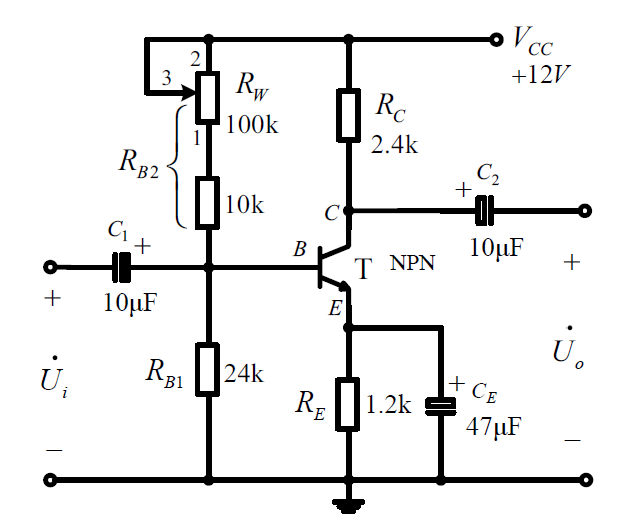
\includegraphics[width=0.5\linewidth]{static.PNG}}
    \caption{测量静态工作点电路图}
    \label{fig:static}
    \end{figure}
\subsection{实验内容2}
利用毫伏表与示波器测量电压放大倍数。
\subsection{实验步骤2}
调节函数信号输出器为正弦波形,频率为$1kHz$,并根据毫伏表调节函数信号输出器电压有效值为$u_i=10mV$。
测量电路仍如图 \ref{fig:static}所示,用毫伏表测量输出电压并记录,后用示波器观察输入输出相位关系,画出波形图。
第一次测量时不接入负载$R_L\rightarrow\infty$,第二测量时接入$R_L=2.4k\Omega$负载。
\subsection{实验内容3}
测量输入电阻和输出电阻。
\subsection{实验步骤3}
在输入端接入$R=2k\Omega$电阻,实验电路图调整为如图 \ref{fig:inAndOutR}所示。测量相应的$U_s,U_i$并计算出输入电阻。
后测量此时的输出电压$U_L$, 断开负载,测量此时的电压$U_o$,由此计算出输出电阻。(注意保持输入信号大小不变)
\begin{figure}[htbp]
  \centering
  \fbox{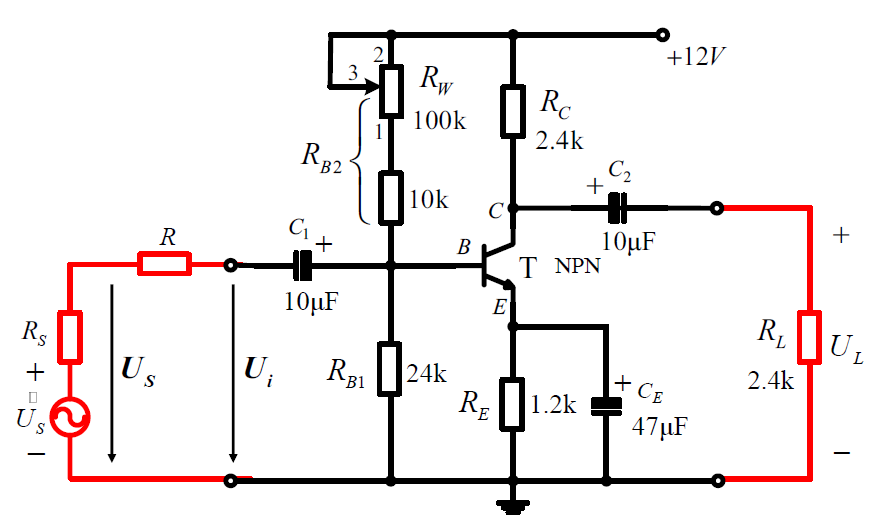
\includegraphics[width=0.5\linewidth]{inAndOutR.PNG}}
  \caption{测量输入输出电阻电路图}
  \label{fig:inAndOutR}
  \end{figure}

\subsection{实验内容4}
测量放大电路通频带。
\subsection{实验步骤4}
将测量电路改回至图 \ref{fig:static}所示。保持输入电压有效值$U_i=10mV$。调整输入频率,直到输出有效值最大,记录此时的输出电压$U_L$。保持输入电压不变,调整输入频率,分别向上向下调至$U_o=U_L/\sqrt{2}$,分别
记录$f_H,f_L$。
\section{实验数据处理与分析}
\subsection{实验内容1}
	实验测得的静态工作点参数为$U_B=3.019V,U_{CE}=4.862V, I_C=2.000mA$。
\subsection{误差分析1}
  采用一般的射级偏置电路分析方法,取$U_{BE},R_{B2}$为测量值,所有原件标记值认为四位有效数字真值,有
  \begin{equation}
    \begin{aligned}
      U_{BQ}&\approx V_{CC}\frac{R_B1}{R_B1+R_B2}=3.215V\\
      I_{CQ}&\approx I_{EQ}\approx\frac{V_{BQ}-V_{BEQ}}{R_e}=2.163mA\\
      U_{CEQ}&=V_{CC}-I_{CQ}(R_e+R_c)=4.2132V
    \end{aligned}
  \end{equation}
  则由此可以计算出三者的相对误差分别为$\left |\frac{\Delta U_B}{U_{BQ}}\right |=6\%,\left |\frac{\Delta I_C}{I_{CQ}}\right |=8\%,\left |\frac{\Delta U_{CE}}{U_{CEQ}}\right |=15\%$。
  由此可见,静态工作点误差普遍较大,但在实验精度范围内可以接受,误差主要来自于两个方面:
  \begin{enumerate}
    \item 万用表测量的精度有限,接线时存在接触电阻,导致存在测量误差;
    \item 原件真实值与标记值存在差异,同时在理论计算中存在一定的近似,因此计算所得到的理论值可能有较大偏差。
  \end{enumerate}
  因此,此次的测量结果还是认为是符合要求的。
  \subsection{实验内容2}
  实验所测得的电压放大倍数在有负载和负载断路时的值分别为$A_{vo}=-148,A_{vL}=-70$。相位从示波器上观察,在精度范围内,都是比较严格的反向,负载断路时波形图如附图所示。
  \subsection{误差分析2}
  同样,静态工作点值采用实验内容1中测量所得的值,$\beta=150,r_b=300\Omega$,由此计算增益系数如下:
  \begin{equation}
    \begin{aligned}
      r_{bet}&=r_{b}+(1+\beta) \frac{26(mV)}{I_E(mA)}=2.263k\Omega\\
      A_{vot}&=\frac{-\beta R_{c}}{r_{be}}=-159.0\\
      A_{vLt}&=\frac{-\beta R_{c}\parallel R_{L}}{r_{be}}=-79.54
    \end{aligned}
  \end{equation}
  由此可以计算出相对误差分别为$\left |\frac{\Delta A_{vo}}{A_{vot}}\right |=7\%,\left |\frac{\Delta A_{vL}}{A_{vLt}}\right |=12\%$。可见误差仍然是比较大,即使在计算时采用了
  实验测得的静态工作点值,原因在于小信号模型本身就是一种近似处理,同时原件的标记值可能有一定的误差。还注意到波形时,实际上上下波形并不对称,这也是由于小信号模型本身属于一种近似处理导致的。
  还可以观察到,空载和加了负载时的电压放大系数理论上应为严格的两倍关系,但测量出的结果并不如此,可能出现了一定的信号失真,可能涉及到耦合电容对其的作用,在此处的理论计算也没有考虑进去,因此,这样的处理和测量获得的值还是可以认为是合理的。

  \subsection{实验内容3}
  实验测量得到的输入和输出电阻分别为$R_i=2.48k\Omega,R_o=2.43k\Omega$。
  \subsection{误差分析3}
  采用实验测得的静态工作点值,计算得到的输入输出电阻如下:
  \begin{equation}
    \begin{aligned}
      R_{it}&=R_{B1}\parallel R_{B2}\parallel r_{be}=2.00k\Omega\\
      R_{ot}&\approx R_{c}=2.40k\Omega
    \end{aligned}
  \end{equation}
  相对误差分别为$\left |\frac{\Delta R_{i}}{R_{it}}\right |=24\%,\left |\frac{\Delta R_{o}}{R_{ot}}\right |=1\%$。可见输入电阻的测量误差惊人得大,而输出电阻却惊人的小。对比差异,考虑到$C_e$对输入电阻的计算影响较大,而对输出电阻计算的影响较小,
  推测是由于计算时忽略了$C_e$带来的误差,小信号模型应本身存在一定的近似误差。而$R_{o}$符合得比较好,误差应该是主要由于忽略了$r_{ce}$造成的,同时也有不可忽视的测量误差。
  \subsection{实验内容4}
  实验测量得到的截止频率分别为$f_L=328Hz,f_H=840Hz$,通频带为$328-840Hz$
  \subsection{误差分析4}
  下面理论计算其下截止频率,此时耦合电容不可忽略(参考模拟电路中的算法),应有两个转折频率:
  \begin{equation}
    \begin{aligned}
     C_1&=\frac{C_1C_E}{(1+\beta)C_1+C_E}=0.3019\mu F\\
     f_{L1}&=\frac{1}{2\pi C_1(R_S+r_{be})}\approx 233Hz\\
     f_{L2}&=\frac{1}{2\pi C_2(R_c+R_L)}\approx 3.316Hz
    \end{aligned}
  \end{equation}
  由于两者相差四倍以上,取$f_{L1}=233Hz$为下限频率,实验实际测得为$328Hz$,相对误差为$41\%$,误差相当大,但此处的理论计算有大量的近似
  处理,导致实际计算出的值比较不精确,因此可以接受。
  高频计算估计如下:
  \begin{equation}
    \begin{aligned}
      R&\approx r_{be'}\parallel(r_{bb'})=260\Omega\\
      C&=C_{b'e}+(1+g_m R_L')C_{b'c}\approx 1.03 nF\\
      f_H&=\frac{1}{2\pi RC}=594kHz
    \end{aligned}
  \end{equation}
  此处的相对误差也非常大,但三极管的具体参数其实并不明,此处采用的参数基本上是估计值,因此数量级是吻合的,可以认为数据没有问题。
\section{实验总结}
本次实验用过理论与测量结合,分析了分压式共射极电路的静态工作点,放大系数以及频率响应,尽管理论与实验测量所得结果误差较大,但仍在实验精度可以接受的范围内,
因此,此次的测量结果还是认为是符合要求的。同时学习到了三极管的小信号分析方法,以及高频响应模型的相关原理,获益匪浅,可以认为本次实验结果较为令人满意。
\section{实验思考题}
balabalabala

\begin{appendix}

\section{代码示例}

\begin{lstlisting}[caption={一段C代码},captionpos=b]
#include <stdio.h>
int main (int argc, char *argv[]){
  printf("Hello world!");
}
\end{lstlisting}

\section{表格示例}
表 \ref{tab:tab1}与表 \ref{tab:tab2}展示了表格示例
\begin{table}[!h!tbp]
\caption{一个简单的表格}\label{tab:tab1}
  \centering
  \begin{tabular}{|l|c|c|}
	\hline
	功能          &WEB         &APP         \\ \hline
	注册          &$\surd$     &$\surd$     \\ \hline
	登录          &$\surd$     &$\surd$     \\ \hline
	推送          &$\times$    &$\surd$     \\ \hline
\end{tabular}
\end{table}

\begin{table}[!h!tbp]
\caption{自定义表格}\label{tab:tab2}
  \centering
\begin{tabular*}{0.75\textwidth}{@{\extracolsep{\fill}}lcc}
    \toprule
    功能          &WEB         &APP         \\
    \midrule
    注册          &$\surd$     &$\surd$     \\
    登录          &$\surd$     &$\surd$     \\
    推送          &$\times$    &$\surd$     \\
    \bottomrule
\end{tabular*}
\end{table}


\section{图片示例}
图 \ref{fig:logo}展示了一个图片示例。
\begin{figure}[htbp]
\centering
\fbox{
\includegraphics[width=0.5\linewidth]{logo}}
\caption{blablabla}
\label{fig:logo}
\end{figure}

\section{公式示例}
式 (\ref{eqa:01})展示了一个公式的例子。
\begin{equation}
S_n = \frac{X_1 + X_2 + \cdots + X_n}{n}
      = \frac{1}{n}\sum_{i}^{n} X_i
\label{eqa:01}
\end{equation}




\end{appendix}

\end{document}
